\documentclass[10pt,twocolumn]{article}
\usepackage[a4paper, left=1.5cm, right=1.5cm, top=2cm, bottom=3cm]{geometry}
\usepackage[T1]{fontenc}
\usepackage[utf8]{inputenc}
\usepackage[italian]{babel}
\usepackage{amsmath}
\usepackage{titling}
\usepackage{caption}
\usepackage{graphicx}
\usepackage{float}
\usepackage{relsize}
\usepackage{amsmath}
\usepackage{sectsty}
\usepackage{ragged2e}
\usepackage{circuitikz}
\usepackage{booktabs}
\usepackage{enumitem}
\usepackage{tikz}
\usepackage{physics}
\usepackage{xcolor}
\usepackage[most]{tcolorbox}
\usepackage{tikz-3dplot}
\usepackage{tikz}
\usepackage{ragged2e}
\usepackage{siunitx}
% \usepackage{booktabs}
\usepackage[colorlinks=true, linkcolor=black]{hyperref}  %per rendere l'indice genrale "interattivo"
\usepackage{enumitem}  %distanza degli itemize
\setlist[itemize]{itemsep=4pt, parsep=1pt}
\newtcolorbox{nota}{
  blanker,
  before skip=1em,
  after skip=1em,
  left=1em,
  borderline west={1pt}{0pt}{black},
  fontupper=\itshape,
  before upper={\noindent\textbf{Nota}:\quad}
}



\begin{document}
\justifying
	\title{\textbf{Misura della curva volt-amperometrica di una lampadina a filo di tungsteno}}
	\author{Brusini Alessio \hspace{0.7cm} Ferrari Carola \hspace{0.7cm} Mirolo Manuele \hspace{0.7cm} Stroili Emanuele}
	\date{14 Ottobre 2025}
	\maketitle
	\newgeometry{left=3cm, right=3cm, top=4cm, bottom=4cm}
	\onecolumn
	\tableofcontents
\vspace{3cm}
	\begin{abstract}
		\centering
		\large
    L'esperimento consiste nell'ottenere la curva volt-amperometrica di una 
    lampadina a filamento, partendo da tensioni basse fino alla fusione del 
    tungsteno. L'obiettivo è verificare l'andamento non ohmico della resistenza
    interna della lampadina, 
       
	\end{abstract}

	\newpage
\restoregeometry
\twocolumn

\section{Apparato sperimentale}
\subsection{Misura per bassi voltaggi}
Per ottenere la misura a bassi voltaggi si costruisce un circuito composto da:
\begin{itemize}
    \item Generatore di corrente continua
    \item Resistenza 
    \item Voltmetro
    \item Amperometro
    \item Fotodiodo
    \item Lampadina con tensione di funzionamento 6V
\end{itemize}
\begin{center}
\begin{circuitikz}[american]
    
    % Generatore di corrente continua variabile a sinistra
    \draw (0,0) to[battery1, invert, l=$V$] (0,3);
    
    % Resistenza in alto
    \draw (0,3) to[R, l=$R$] (3,3);
    
    % Lampadina a destra
    \draw (3,3) to[lamp, l=$L$] (3,0);
    
    % Amperometro in basso
    \draw (0,0) to[rmeter, t=A] (3,0);
    
    \draw (3,2) to[short] (2,2) 
    % Voltmetro in parallelo alla lampadina
    to[rmeter, t=V] (2,1)
    to[short] (3,1);

    % Fotodiodo in parallelo alla lampadina
    \draw (5,0) to [empty diode, a_=$Photodiode$] (5,3);
\end{circuitikz}
\end{center}
\subsection{Seconda misura}
Per ottenere la misura con gli altri voltaggi si costruisce un circuito composto da:
\begin{itemize}
    \item Generatore di corrente continua
    \item Voltmetro
    \item Amperometro
    \item Lampadina con tensione di funzionamento 6V
\end{itemize}
\begin{center}
\begin{circuitikz}[american]
    
    % Generatore di corrente continua variabile a sinistra
    \draw (0,0) to[battery1, invert, l=$V$] (0,3);

    % Filo conduttore in alto
    \draw (0,3) to (3,3);
    
    % Lampadina a destra
    \draw (3,3) to[lamp, l=$L$] (3,0);
    
    % Amperometro in basso
    \draw (0,0) to[rmeter, t=A] (3,0);
    
    \draw (3,2) to[short] (2,2) 
    % Voltmetro in parallelo alla lampadina
    to[rmeter, t=V] (2,1)
    to[short] (3,1);

\end{circuitikz}
\end{center}
\section{Procedimento di misura}
La misura si svolge in due fasi: nella prima si prendono misure più fitte
per poter apprezzare le oscillazioni di corrente. A questo scopo è necessario
introdurre una resistenza nel circuito da utilizzare come partitore di tensione.
Inoltre, nella prima fase, ci si serve di un fotodiodo per poter captare la 
flebile luminescenza della lampadina, non visibile univocamente a occhio nudo.\\
Nella seconda fase si prendono dati meno fitti, perciò si rimuovono la 
resistenza e il fotodiodo dal circuito, non più necessari nella misura.

%\section{Dati}
%\begin{table}[H]+3
%    \begin{minipage}{0.5\textwidth}
%        \centering
%        \caption*{}
%        \label{tab:temp2}
%        \begin{tabular}{|r|r|}
%            \hline
%            Tensione(V) & Corrente (A) \\ \hline
%            0 & 17.2 \\ \hline
%            30 & 17.2 \\ \hline
%            60 & 17.2 \\ \hline
%            90 & 17.2 \\ \hline
%            120 & 17.1 \\ \hline
%            150 & 17.1 \\ \hline
%        \end{tabular}
%    \end{minipage}
%\end{table}

%\twocolumn

\section{Grafici}
\begin{figure}[H] % [h] = here, posizione approssimativa
  \centering
  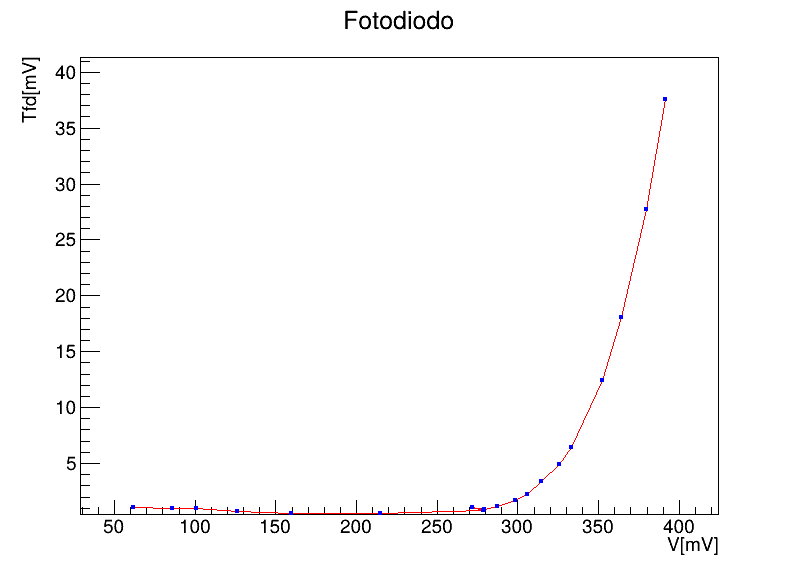
\includegraphics[width=0.5\textwidth]{curva_voltammetrica/fotodiodo.png} % o .png, .pdf, ecc.
  \label{fig:I/V_fotodiodo}
\end{figure}
Nel grafico si può osservare qual è la differenza di potenziale (V) che va applicata alla lampadina per osservare il primo fenomeno soglia, ovvero l'emissione di fotoni dovuta all'eccitazione degli atomi del tungsteno.
%Nel grafico possiamo osservare a quale differenza di potenziale ai capi della mia lampadina (V) si verifica il primo fenomeno soglia, ovvero l'emissione di fotoni. 
Da quel punto in poi la lampadina non avrà più un comportamento ohmnico. Questo è dovuto al fatto che la forza elettromotrice, oltre alla semplice accelerazione degli elettroni, provoca anche l'agitazione termica del filamento di tungsteno, che inizia a riscaldarsi e quindi a emettere luce visibile, dissipando così energia sotto forma di calore. \\
Essendo questo fenomeno non lineare, la resistenza interna della lampadina non sarà più costante, a partire da quel punto. 

\begin{figure}[H] % [h] = here, posizione approssimativa
  \centering
  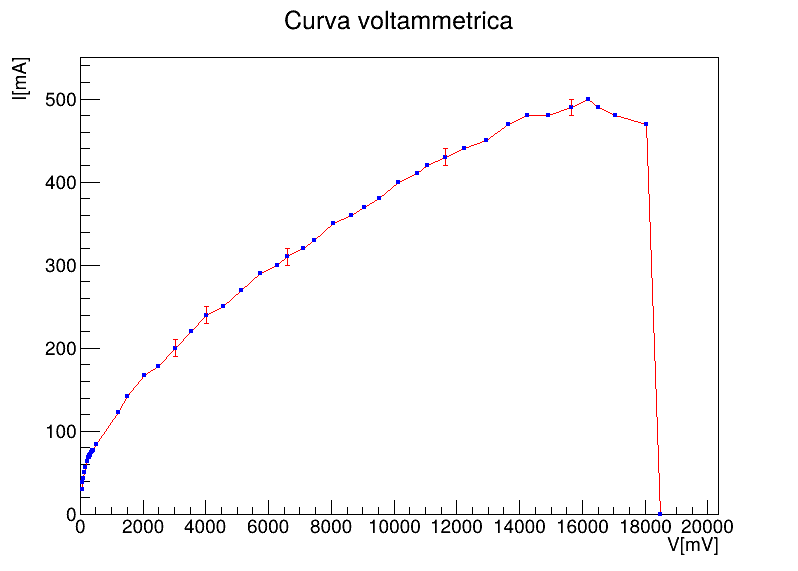
\includegraphics[width=0.5\textwidth]{curva_voltammetrica/curva_voltamperometrica.png} % o .png, .pdf, ecc.
  \label{fig:I_V_}
\end{figure}
Nella curva posso notare due principali regioni:
\begin{itemize}
    \item La prima regione in cui la corrente sembra avere una tendenza del tipo $I \propto V^{1/2}$;
    \item La seconda regione ($V > 14V$), in cui la mia corrente sembra stabilizzarsi all'aumentare della tensione, avendo anche una piccola discesa nella parte finale;
\end{itemize}
Andiamo ora a presentare il grafico rispetto al valore sotto radice quadrata della tensione:
\vspace{1.5cm}
\begin{figure}[H] % [h] = here, posizione approssimativa
  \centering
  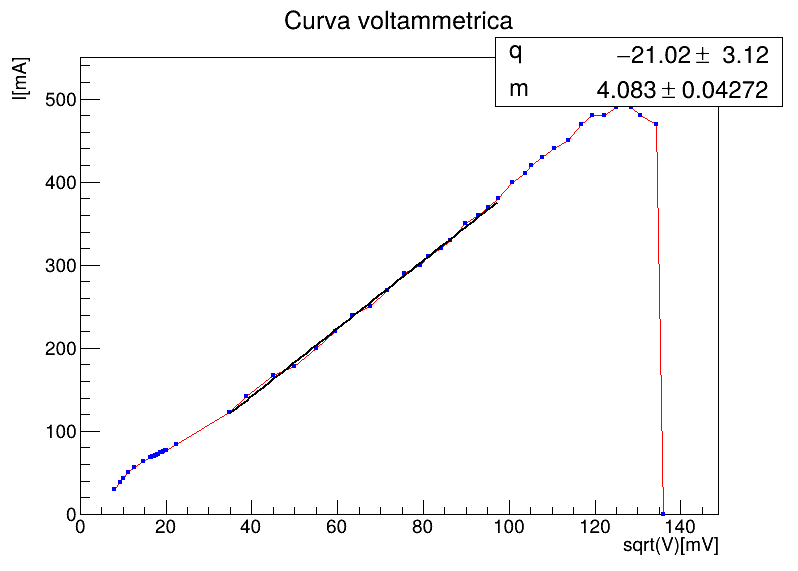
\includegraphics[width=0.5\textwidth]{curva_voltammetrica/curva_voltammetrica_sqrt.png} % o .png, .pdf, ecc.
  \label{fig:I_V_}
\end{figure}
\noindent Costruendo un grafico in cui si riportano la radice quadrata della tensione in ascissa e l'intensità di corrente in ordinata, si possono osservare meglio le due zone precedentemente descritte.
%Andiamo ora a presentare il grafico rispetto al valore sotto radice quadrata della tensione:
In particolare si nota la dipendenza quadratica dell'intensità di corrente rispetto alla tensione nel range $400-13000mV$.\\ 
%Nella regione iniziale si osserva un andamento che può essere ricondotto ad un'esponenziale.
%Questa cosa dell'esponenziale ha senso dirla?


\begin{figure}[H] % [h] = here, posizione approssimativa
  \centering
  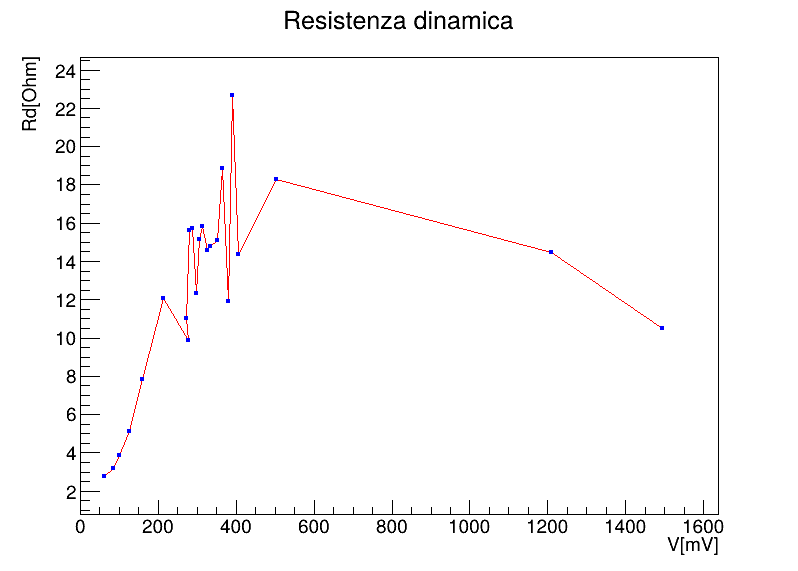
\includegraphics[width=0.5\textwidth]{curva_voltammetrica/resistenza_dinamica_zoom.png} % o .png, .pdf, ecc.
  \label{fig:I_V_}
\end{figure}
 In questo grafico è rappresentata la resistenza dinamica (calcolata come $\Delta V/\Delta I$) in funzione del voltaggio. La prima parte del grafico è quasi nulla, mostrando come la resistenza a bassi voltaggi rimanga quasi costante, mentre all'aumentare del voltaggio entrano in gioco fenomeni che rendono la resistenza variabile. 
Come ci si aspetta da un filamento che si riscalda, la resistenza dinamica tende ad aumentare.
%Quello che mi interessa è il fatto che la resistenza dinamica comunque tenda ad aumentare, come ci si aspetta per un filamento che si riscalda.
\begin{figure}[H] % [h] = here, posizione approssimativa
  \centering
  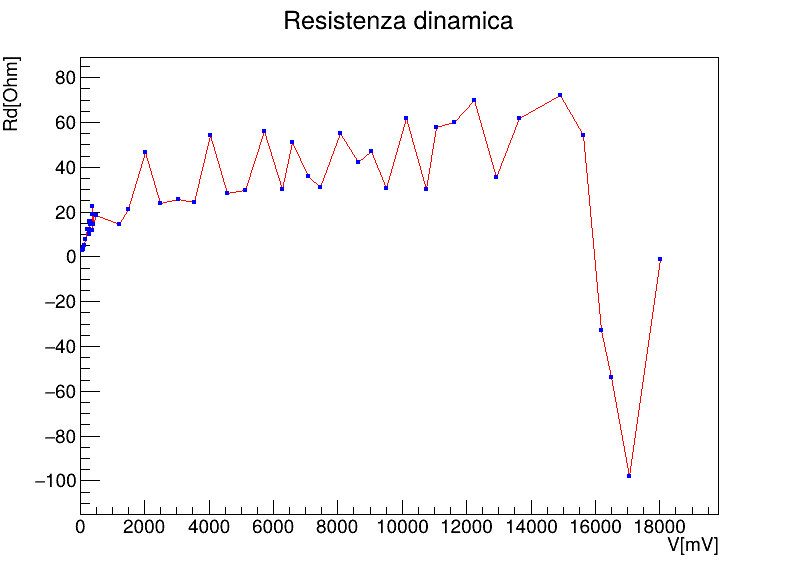
\includegraphics[width=0.5\textwidth]{curva_voltammetrica/resistenza_dinamica.png} % o .png, .pdf, ecc.
  \label{fig:I_V_}
\end{figure}
\noindent Guardando l'andamento generale della resistenza dinamica, si nota come questa oscilli molto; ciò è dovuto al fatto che è stato usato un amperometro con fondoscala di $10 A$, andando ad accumulare molto errore nelle misure.
Infatti per una variazione misurata di $0.1 A$ si presenta un errore sullo strumento altrettanto grande.\\
In generale si riesce ad osservare come la resistenza tenda ad aumentare all'aumentare della tensione, fino a raggiungere un massimo di circa $60 \: \Omega$. 
Da quel punto in poi si osservano delle violente oscillazioni, dovute probabilmente all'inizio della fusione del filamento di tungsteno. 

\section{Conclusione}
Non potendo dare una stima quantitativa per stabilire la riuscita
 dell'esperimento è possibile darne una stima qualitativa: osservando 
 il terzo grafico, come già analizzato in precedenza,
  è possibile notare che l'andamento lineare dei valori di corrente misurata in 
  funzione della radice quadrata della tensione stanno ad indicare come la corrente, 
  per la maggior parte dei dati raccolti, in particolare per il range  $400-13000mV$, 
  abbia proprio andamento $I \propto \sqrt{V}$ che ci si aspettava in virtù del fatto
   che la lampadina sottoposta a valori simili di differenza di potenziale non si comporta in modo ohmico

\end{document}